\documentclass[12pt, final, onecolumn, titlepage]{article}
\usepackage{amsmath}
\usepackage{amsfonts}
\usepackage{amssymb}
\usepackage{enumitem}
\usepackage{titlesec}
\usepackage{listings}
\usepackage[colorlinks = true,
            linkcolor = blue,
            urlcolor  = blue,
            citecolor = blue,
anchorcolor = blue]{hyperref}
\usepackage{leftidx}
\usepackage{amsthm}
\usepackage{mathtools}
\usepackage{comment}
\allowdisplaybreaks
\titlelabel{\thetitle.\quad}
\usepackage[margin=1in]{geometry}

\newcommand{\vect}[1]{\mathbf{#1}}
\newcommand{\re}{\text{Re}}
\newcommand{\imcp}{\text{Im}}
\newcommand{\CC}{\mathbb{C}}
\newcommand{\RR}{\mathbb{R}}
\newcommand{\QQ}{\mathbb{Q}}
\newcommand{\ZZ}{\mathbb{Z}}
\newcommand{\NN}{\mathbb{N}}
\newcommand{\FF}{\mathbb{F}}
\newcommand{\SL}{\text{SL}}
\newcommand{\Hom}{\text{Hom}}
\newcommand{\vol}{\text{vol}}
\newcommand{\const}{\text{const}}
\newcommand{\ord}{\text{ord}}
\newcommand\norm[1]{\left\lVert#1\right\rVert}
\newcommand\abs[1]{\left\lvert#1\right\rvert}
\newcommand\ceil[1]{\left\lceil#1\right\rceil}
\newcommand\floor[1]{\left\lfloor#1\right\rfloor}
\newcommand\parens[1]{\left(#1\right)}
\newcommand*{\pr}[2][]{\text{Pr}\ifx\\\left[#1\right]\\\else_{#1}\fi \left[#2\right]}

\theoremstyle{definition}
\newtheorem{defin}{Definition}[section]
\newtheorem{remark}[defin]{Remark}
\newtheorem{prop}[defin]{Proposition}
\newtheorem{lemma}[defin]{Lemma}
\newtheorem{theorem}[defin]{Theorem}
\newtheorem{corollary}[defin]{Corollary}
\newtheorem{example}[defin]{Example}
\newtheorem{problem}[defin]{Problem}

\begin{document}

\title{Making Fantasy Football Predictions Using Multiplicative Weights}

\author{Dylan Mavrides (\texttt{mavrides})\\Eric Neyman (\texttt{eneyman})\\Andrew Wonnacott (\texttt{awonnacott})}

\maketitle

\tableofcontents

\newpage

\section{Introduction}
The multiplicative weights algorithm, as presented in class, essentially gives a method of making a single good prediction using the predictions of many experts at a series of time steps. To do so, we fix a constant $\eta \leq 1/2$ (for theoretical results to hold), and then we associate weights $w_{i}^{(t)}$ (initialized to 1) for each expert $i$ and time step $t$. At time step $t$ we choose decision $i$ with probability
\[p_i = \frac{w_i^{(t)}}{\sum_{j}w_j^{(t)}}.\]
Now we assume some cost function associated with how incorrect each decision was. Let these costs be $m^{(t)}$, and then update the weights by multiplying them by the factor $1-\eta m_i^{(t)}$.

In the theoretical sense, this algorithm has small additive error asymptotically. However, we wanted to apply the algorithm to a more practical scenario, to see how well the algorithm performed in practice relative to the experts it was using to make predictions. After considering a few different settings in which a bunch of experts make straightforward, publicly-available predictions including weather forecasts and a website where people predict the outcomes of supreme court cases, we settled on fantasy football as our final setting, with ESPN, Fantasydata, Fantasyalarm, Yahoo, CBS, NFL, and FFToday as our experts, making predictions on the number of fantasy points for each player.\footnote{We only looked at quarterbacks (QB), running backs (RB), wide receivers (WR), and tight ends (TE) because for other positions, websites differed in what they factored into fantasy points. Fantasy points are calculated according to a linear combination of passing yards, passing touchdowns, passes intercepted, rushing yards, rushing touchdowns, receiving yards, and receiving touchdowns. The weights we used in the linear combination, for calculating overall fantasy points, were the standard ones: $0.04$, $4$, $-2$, $0.1$, $6$, $0.1$, and $6$, respectively.} We used each week of play in 2017 as our series of time steps, with data for each player in the positions quarterback, running back, wide receiver, and tight end. When a website didn't make a prediction for a particular player, we assumed that this implied a predicted fantasy score of 0. This is a reasonable assumptions, since some websites didn't include players expected not to play, but others included a score of 0 for completeness. To collect our data, we used the python packages Selenium and BeautifulSoup to download the data to CSVs and then write bits of code to standardize the formatting of the data and the names of the players (removing Jr., Sr., and other name suffices).

Since different players play different positions, and different experts may be better or worse at predicting the results of specific positions, we ran different multiplicative weights trials for different sources, as well as an algorithm that disregarded the position itself. Another thing to note is that our algorithm differs slightly from the standard multiplicative weights procedure since we make many updates at each time step, as each expert makes a prediction for each player at each time step. We continued our investigation by seeing which experts seemed more or less credible based on their final weights, adjusting $\eta$ values, and then testing in what way removing the sources that ended up with the worst weights affected our predictions' accuracy.

Of course, in reality, fantasy football involves much more than just predicting the number of fantasy points that each player scores. Importantly, it requires drafting players; according to ESPN.com, this generally includes a quarterback, 2 running backs, 3 wide receivers, one tight end, and a kicker (this may not be exhaustive, and may have some variation among leagues, but this is the setting we will consider). We finish the paper by investigating the theoretical question: given that we have predictions about how the players will perform, how can we maximize our expected chances of winning a fantasy football league?

Through our investigation we found ESPN to be the  best-scoring expert using our metrics, that the multiplicative weights algorithm generally (with reasonable $\eta$) performed better than any expert individually, that it performed a small amount better than simply averaging the experts' predictions ($\eta = 0)$, that high $\eta$ was better when we had "bad" sources, but low $\eta$ was better when only "good" sources were used, and various theoretical results. Finally, we note that we did use relatively few experts, so any conclusions we reach may not necessarily generalize to multiplicative weights when applied to larger-scale settings.

\section{Algorithm Details}
We made two separate algorithms. The first one ran multiplicative weights once: for each week, it calculated a cost for each source, taking into account, for each player, the source's prediction for number of fantasy points for that player and the true number of fantasy points scored. The second algorithm ran four different multiplicative weights algorithms --- one for each of the four positions (QB, RB, WR, TE). The theory was that the latter algorithm would outperform the second one if some sources were better at some positions and other sources were better at other positions, and would just add noise otherwise.

The costs were calculated straightforwardly. For each expert, for each player, that player's cost was the absolute difference of their points scored and the expert prediction for their points scored. This makes sense: suppose you are choosing between two players to draft; an expert says that the first player is expected to score $M - \epsilon$ points and the second player is expected to score $M$ points. You choose the second player; it turns out that actually the second player ends up scoring $m$ points. By choosing the second player, you were hurt by an expected (approximately) $M - m$ points (assuming the predictor does not consistently overshoot or undershoot). (Choosing $\epsilon$ to be small was arbitrary, but it still makes sense that you would be hurt in proportion to the absolute difference between the actual score and the predicted score.) Then, these costs were summed across all players, giving the expert's total cost. This number was scaled to lie between $-1$ and $1$.

The method of scaling was as follows: there was some constant margin $t$ (specifically, $t = 1.3$). Suppose that the first week's costs are $c_1 < \dots < c_n$, where there are $n$ sources. If all future costs lie between $\frac{c_1}{t}$ and $c_nt$, we can ensure that all costs are between $-1$ and $1$ by linearly scaling the costs $c \mapsto ac + b$, where $a$ and $b$ are such that $\frac{c_1}{t}$ maps to $-1$ and $c_nt$ maps to $1$. Specifically, this gives us:
\[a = \frac{2}{c_n t - \frac{c_1}{t}}; b = 1 - ac_nt.\]
In practice this does not always ensure that the costs lie between $-1$ and $1$ (though they are close to always lying in that range); however, we are not trying to prove theoretical results so this is fine.

\section{Analysis of Results}
The most important takeaway from our results is that the multiplicative weights approach passes two basic tests. First, even though ESPN was consistently the best expert, the multiplicative weights algorithm performed better than ESPN by itself. With $\eta = \sqrt{\frac{\ln n}{T}}$ (the default $\eta$ since this is the $\eta$ used in the theoretical result), the total accumulated cost of the algorithm was $2.7\%$ better than just ESPN's predictions.

Second, the approach was better than simply taking an average of all predictors each week (equivalently, setting $\eta = 0$), by $0.34\%$. The primary reason for that this percentage seems small is that sources' predictions were all fairly similar to each other, so although some sources were consistently better than others, they weren't better than others by large absolute amounts.

Note that we did not specify whether we were talking about the overall algorithm or the by-position algorithm (that runs multiplicative weights algorithms for each position). This is because these two algorithms always performed about equally well. In the standard setting (default $\eta$, all sources present), for instance, the by-position algorithm was better than the overall algorithm by just $0.042\%$. Our hypothesis for this result is that the amount by which sources had weak suits and strong suits in terms of positions (existent but not large) roughly cancelled out the negative effect we would expect from noise (having less data each week to update weights based on), resulting in similar performance. For a sense of the extent to which experts had strong and weak suits, see the table below. The table shows the final weights assigned to each source (scaled so the highest weight is $1$) in the overall algorithm and the by-position algorithm.
\begin{center}
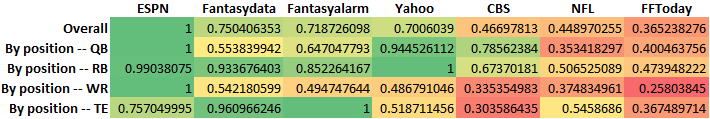
\includegraphics[scale=0.8]{Scaled_Weights.png}
\end{center}
Because the algorithms always performed comparably well, no matter the specific settings, from now on we will analyze the performance of the overall algorithm without mentioning how the by-position algorithm did.

Another question is, while excluding all sources besides ESPN made things worse, perhaps excluding bad sources like FFToday would be beneficial. And indeed, excluding bad sources does make the algorithm do better. Below, we exclude sources starting from the worst overall one above (FFToday) up to the second best one (Fantasydata).

\begin{center}
\begin{tabular}{|r|l|}
\hline
Sources & Total Cost\\
\hline
FFToday, NFL, CBS, Yahoo, Fantasyalarm, Fantasydata, ESPN & 19499\\
NFL, CBS, Yahoo, Fantasyalarm, Fantasydata, ESPN & $19476$\\
CBS, Yahoo, Fantasyalarm, Fantasydata, ESPN & $19338$\\
Yahoo, Fantasyalarm, Fantasydata, ESPN & $19204$\\
Fantasyalarm, Fantasydata, ESPN & $19198$\\
Fantasydata, ESPN & $19356$\\
ESPN & $20047$\\
\hline
\end{tabular}
\end{center}
That is, it seems that a medium number of sources is optimal: bad sources should be excluded but it is suboptimal to only include the best source.

Interestingly, the optimal combination of sources actually appears to be just ESPN and Fantasyalarm, with an overall cost of $19176$. Perhaps ESPN and Fantasyalarm complement each other in some way. One conjecture would be that ESPN is better for quarterbacks, running backs, and wide receivers, while Fantasyalarm is better at tight ends (see the table with scaled weights), which is why it is good (and sufficient) to have both. However, this is not the correct explanation; if it were correct, we would see the combination of the two doing substantially better in the by-position algorithm. But this is not the case: with a cost of $19168$, the by-position algorithm does only $0.04\%$ better.

Our recommendation would not be to use just ESPN and Fantasyalarm in future years: the performance of these two in combination could just be good by coincidence. Instead, using ESPN, Fantasydata, Fantasyalarm, and Yahoo (all good sources, unlike CBS, NFL, and FFToday), would result in online correction of any potential overfitting due to the above model.

Another question is, what is the optimal $\eta$? Below is a chart showing total cost for various values of $\eta$, for both all sources and just the four best ones. (Note that for all sources included, the theoretical $\eta = \sqrt{\frac{\ln n}{T}}$ is about $0.34$, while for four sources it is about $0.29$.)
\begin{center}
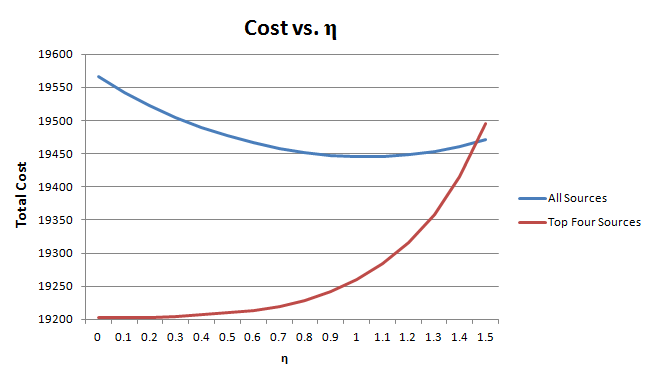
\includegraphics[scale=0.7]{Cost_vs_eta.png}
\end{center}
One should not read too much into the \emph{specific} values of $\eta$, because the specific value of $\eta$ depends entirely on how we scale our costs. However, the fact that multiplicative weights with all sources prefers a higher $\eta$ makes sense. Because there are sources of varying quality, a higher $\eta$ quickly reduces the weight of the bad sources. On the other hand, when there is not much quality differentiation (as is the case if we take the top four sources), a low $\eta$ is optimal. Indeed, setting a very high $\eta$ results in nearly all the weight being put on ESPN ($78\%$ of the weight for $\eta = 1.5$), which is close to the case where ESPN is our only source (which does poorly).

\section{Trying to Win: A Theoretical Approach}
Suppose that your fantasy football league has the following format: each week, the person with the largest total number of fantasy points wins a cash prize (everyone else gets nothing). If you wish to maximize your prize money, then each week you wish to maximize the probability that you will come in first. Maximizing expected score given a belief about how many points each player is expected to score is easy: by linearity of expectation, the optimal approach is to pick the top quarterback(s), the top running back(s), etc. Maximizing probability of winning is not so straightforward: sometimes it might make sense to maximize expectation for variance. In this section, we create a simplified model of fantasy football and analyze how to maximize the probability of winning in a given week.

Suppose there are $n$ people in your league, not including you. Assume that everyone else has the na\"{i}ve strategy of trying to maximize their expected number of points. What is the maximum of their fantasy points expected to look like? One reasonable model is to model each person's point distribution as a normal distribution centered at some $\mu$ with standard deviation $\sigma$. After all, the random variable of each person's points is a sum of the random variables that are the number of fantasy points each player on that person's fantasy team scores; it makes sense for these to be jointly normally distributed, and the sum of jointly normally distributed random variables if a normally distributed random variable. We assume that $\mu$ and $\sigma$ are the same for all $n$ players: the snake draft system makes it so that equally skilled players get roughly the same expectation, and it seems likely that in practice the standard deviations won't be too different from each other.

Furthermore, we will assume that these $n$ normal random variables are independent. This makes sense because everyone has different players, and although e.g. two players on the same team are likely to have positively correlated points, this is unlikely to be a significant effect unless two people both have several players all drawn from the same team. So now our question is, how is the maximum of $n$ independent random variables $N(\mu, \sigma)$ distributed?

Let $p(x)$ and $c(x)$ be the PDF and CDF of $N(\mu, \sigma)$, respectively. The probability that the maximum of the $n$ random variables is less than $t$ is just the product of the probabilities that each of the random variables is less than $t$, i.e. $c(t)^n$. This is the CDF of the maximum of the random variables. The PDF, while not immediately relevant to the problem, is interesting. It is
\[nc(t)^{n - 1}c'(t) = nc(t)^{n - 1}p(t),\]
which looks similar to a normal distribution, but is skewed (the larger the value of $n$, the more skewed it is). Here is a picture for $n = 10$ (with $\mu = 0$ and $\sigma = 1$):
\begin{center}
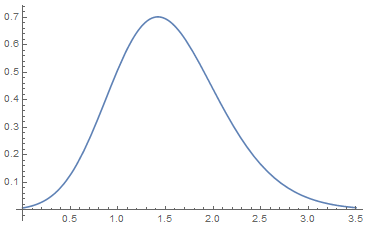
\includegraphics[scale=0.7]{Maximum_Distribution_N=10.png}
\end{center}

Now, if you know the distribution of your possible scores, finding the probability that you will be the week's winner is straightforward. (You can write the exact answer as an integral, or you can approximate the probability that you will be the winner: finely subdivide the $x$-axis into regions $[-\infty, x_0), [x_0, x_1), \dots, [x_r, \infty)$, and for each $0 \le i < r$, take the probability that your score is in $[x_r, x_{r + 1})$ times the $c(x_r)^n$, and add up these products.) We now discuss how you can calculate your distribution of possible scores, given the list of players.

As we said before, the football players' scores are jointly normally distributed. However, we cannot assume that they are independent: indeed, the point of the question is how much expectation should be given up to exploit non-independence for increased variance.

Suppose that we have a list of all of the football players $p_1, \dots, p_m$ with mean fantasy scores $\mu_1, \dots, \mu_m$ (found e.g. from expert predictions via multiplicative weights). There is an associated covariance matrix $\Sigma$ (where the entry $\sigma_{ij}$ is the covariance of $p_i$'s fantasy score and $p_j$'s fantasy score). The matrix $\Sigma$ can be found empirically by examining how much variance individual players have (to determine the diagonal entries), how much a quarterback's performance affects the performance of a wide receiver on the same team, how scores of players on opposing teams are correlated, etc.

Suppose that the players that you choose are $p_{a_1}, \dots, p_{a_s}$. From statistics we know that the distribution of your total score has mean $\mu_{a_1} + \dots + \mu_{a_s}$ and variance $\sum_{1 \le i, j \le s} \sigma_{a_ia_j}$.

So now, given a set of players that you select, it is easy to find the probability that you will win (under our assumptions). And any given week, it is easy to simply check all sets of players: among the $16$ or so players that you drafted, there are only a few hundred options for whom to select. However, it is still useful to examine the question of which players you should select in full generality (i.e. if you could select any of the players), for two reasons: first, opportunities for trades; and second, in order to know whom to draft in the first place. There are too many possibilities to brute force this more general problem.

Suppose for the moment that your goal is to maximize the probability that you score better than some score $N$. Then equivalently, you want to maximize the number of standard deviations above the mean of your distribution of possible scores that $N$ is. That is, you are trying to minimize
\[\frac{N - \sum_{i \in [s]} \mu_{a_i}}{\sqrt{\sum_{i, j \in [s]} \sigma_{a_ia_j}}}.\]

This can be phrased as a minimization problem with variables and constraints by letting $x_k$ be $1$ if $k \in \{a_i\}$ (for $k \in [m]$) and $0$ otherwise, where sums of certain $x_k$'s (those corresponding to quarterbacks, those corresponding to running backs, etc.) have to equal certain numbers. Then we are trying to minimize
\[\frac{N - \sum_{i \in [m]} x_i \mu_i}{\sqrt{\sum_{i, j \in [n]} x_i x_j \sigma_{ij}}}.\]
This minimization problem is not easily approachable. Not only is it an integer program, but its natural relaxation (letting $x_i$ be in $[0, 1]$) is not a convex program: the function we wish to minimize is not convex. For example, let $m = 2$, $N = 1$, $\mu_1 = \mu_2 = 0$, $\sigma_{11} = \sigma_{22} = 1$, $\sigma_{12} = \sigma_{21} = 0$. Then the function is $\frac{1}{\sqrt{x_1^2 + x_2^2}}$, which is not convex (consider $(x_1, x_2) = (1, 0)$, $(x_1, x_2) = (0, 1)$, and their midpoint). Despite this, we can approximate the solution to the minimization problem fairly accurately under certain assumptions.

The main assumption we need is the following: if we arrange the players $p_1, \dots, p_m$ by team (each team has the same number of players in the list) and consistently arrange the players by position within each team, then the covariance matrix $\Sigma$ can be closely approximated by a matrix of the following form:
\[\Sigma_M = \begin{pmatrix}M&0&\dots&0 \\ 0&M&\dots&0 \\ \vdots & \vdots & \ddots & \vdots \\ 0 & 0 & \dots & M\end{pmatrix}.\]
Here, the number of rows (and columns) in $M$ is equal to the number of players on each team. Furthermore, $M$ is a symmetric matrix with the following property: for any player of position $A$ and any other player of position $B$ (where $A$ could equal $B$), the entry for those two players in $M$ is the same as for any other pair of players with positions $A$ and $B$.

It makes sense that $\Sigma$ can be approximated in this way. First, a player from one team and a player on another team should clearly have uncorrelated performances (unless they are on opposing teams, and even then it is not obvious that they ought to be correlated; we discuss taking correlations between opposing players into account later). Second, it does not seem far removed from reality that e.g. the performance of the Patriots quarterback should be correlated with the performance of a Patriots wide receiver in a similar way to how the performance of the Seahawks quarterback should be correlated with the performance of a Seahawks wide receiver. Furthermore, the performance of e.g. a Patriots quarterback and a Patriots wide receiver should be correlated similarly to the quarterback and a different wide receiver.

Note that approximating $\Sigma$ with the closest possible such matrix $M$ is easy. We have a certain number of variables $y_1, \dots, y_q$ corresponding to the distinct entries of $M$; we are trying to minimize a sum of the form $(y_i - \sigma_{jk})^2$, which is a sum of quadratics in each variable, so we can just minimize each variable's quadratic separately.

Now, suppose we take a particular distribution of positions among unlabeled teams. For example, one distribution of \{1 QB, 2 RB, 3 WR, 1 TE, 1 K\} among unlabeled teams is \{\{1 QB, 1 RB\}, \{1 RB, 1 WR\}, \{2 WR, 1 K\}, \{1 TE\}\}, which means that the quarterback and one running back are drawn from one team, the other running back and one wide receiver are drawn from a different team, and so on. If we use $\Sigma_M$ as our covariance matrix, this distribution uniquely determines the denominator of the function we are trying to minimize. This is clear from the properties of $M$.

So suppose we have a particular distribution we want among unlabeled teams. With one caveat, determining \emph{which} teams (and players) to assign to which of the subsets is a straightforward task. Indeed, since the denominator is fixed, we want to minimize the numerator, i.e. maximize $\sum_{i \in m} x_i\mu_i$. For each subset (of the distribution), for each team we find the expected scores of its top players with positions as dictated by the subset, and take players from the team with the highest expected sum of scores. For example, if the Patriots have highest expected score of their two two wide receivers and top kicker among any team, the Patriots would be chosen for the third subset in the example in the previous paragraph.\footnote{This has the obvious problem of selecting the same player multiple times. A way to deal with this is, whenever there are e.g. wide receivers in different subsets, consider the top few choices for those subsets and pick the best valid set of choices.} This is always optimal. So what we do is, cycle through all possible distributions among unlabeled teams (there aren't that many; for eight players the number of distributions is bounded above by the eighth Bell number ($4140$) and is probably substantially lower since there are multiple wide receivers and running backs). For each distribution, calculate the optimal (smallest) value of the function we are trying to minimize. The select the distribution for which the function achieves its smallest value.

The caveat is that perhaps some of the teams assigned to the subsets are not distinct. This is bad because then our calculation for the denominator of our minimization function is wrong, since we do not consider the covariances between players on the same team but in different subsets. There are two ways to address this concern. The first is to point out that it is unlikely to happen for the optimal distribution of players among unlabeled teams. Indeed, most players on the same team are positively correlated. So if e.g. the quarterback and the tight end are in different subsets but end up being drawn from the same team, this ``dishonest" selection actually \emph{undersells} the goodness of the selected players, because after factoring in the cross-subset covariance the denominator of the minimization function will increase.

The second is to create a workaround. For example, invalid arrangements (ones where subsets are assigned to the same team) could be ignored. Or, if an arrangement is invalid, bump conflicting subsets down until there is no longer a conflict. This would most likely produce a near-optimal result.

Finally, we briefly come back to the fact that opposing teams' scores might be correlated. This has a simple fix: instead of letting $M$ have dimension equal to the number of players on each team, it has dimension equal to twice the number of players on each team, and teams are arranged so that opposing teams in a given week are consecutive. Now $\Sigma_M$ can more fully capture all of the covariance in $\Sigma$. However, now there are more distributions of players among unlabeled teams to consider. For example, one such distribution would be \{\{1 QB, 1 RB on opposite teams\}, \{1 RB, 1 WR on the same team\}, \{2 WR, 1 K with one WR on one team and one WR and one K on the opposing team\}, \{1 TE\}\}.

\section{Further Research}
One issue with multiplicative weights that comes to mind is, suppose that we clone a source. Then effectively the weight of that source nearly doubles. In practice, if two experts make similar predictions (which could be if for example they consult each other, or rely on the same techniques), this would cause a multiplicative weights approach to be biased toward those experts/techniques.

One obvious solution to this problem would be to apply known techniques in optimization for post-hoc feature selection, for instance forward and backward stepwise feature selection. In the former, we begin with no approved experts, and then iteratively adopt into our set of approved experts the non-approved expert who would decrease our cost (of running MW on the approved experts) the most, until no non-approved experts provide substantial cost decreases. In the latter, we begin with no rejected experts, and then iteratively eject the expert who would increase our cost (of running MW on the remaining experts) the least, until all remaining experts make substantial contributions to our cost minimization.

However, these techniques sacrifice one of the key advantages of multiplicative weights --- online learning. That is, the multiplicative weights algorithm does not require training to cease in order to make predictions, so there is no requirement of a training vs testing set of data to be drawn from the historical data. When post-hoc feature selection techniques are employed, they introduce the necessity of an out-of-sample data set on which to evaluate performance in order to prevent overfitting to the training data. We did not select to explore this because of the limited data set to which we had access. Readers with more historical data (produced either by the passage of time or by access to data previous to 2017) could explore the applicability of such techniques.

Given these drawbacks, it would be preferable to adapt the multiplicative weights algorithm itself to incorporate feature selection. Two approaches come to mind. First, instead of simply penalizing each expert based on costs, experts' weights could be penalized for proximity to other experts in their predictions. Second, instead of penalizing weights, experts could be penalized in a given round when their predictions are similar to others' predictions (i.e. their predictions are discounted when making the guess), without affecting the experts' weights. An interesting question would be to design an algorithm that does this, perhaps one satisfying certain interesting or useful theoretical properties. (One such property might be that if an expert is duplicated, the predictions of the algorithm do not change.)

Finally, as stated above, we were limited to only using data in 2017 and only seven sets of expert predictions since we wanted to have as complete and consistent data as possible across our sources. To avoid problems with overfitting\footnote{While multiplicative weights is specifically designed to protect against overfitting (by only using past data to predict future data), throwing out bad sources in retrospect produces results that are subject to overfitting.} and further legitimize our results, we would ideally use more data from past years and continue using our algorithm to make predictions in future years as the sites make more predictions. In a real-life setting, if we were trying to provide a service of fantasy football predictions, it would be useful to automate this process and add protocols to the algorithm to incorporate new experts as we find more sources from which to make predictions.
\newpage
\appendix
\section{Code}
Relevant constants (in clean\_data.py, which contains a clean method which returns a two-dimensional array containing players of a given position along with predicted scores for each statistics, e.g. passing yards, passing touchdowns, etc.):

\footnotesize
\begin{lstlisting}[basicstyle=\small\ttfamily,breaklines=true,breakatwhitespace=true,language=Python]
experts = ["espn", "nfl", "fftoday", "cbs", "fantasydata", "fantasyalarm", "yahoo"]
positions = ["QB", "RB", "WR", "TE"]
num_weeks = 17
points_weights = [.04, 4, -2, .1, 6, .1, 6]
\end{lstlisting}

\normalsize
\noindent Multiplicative weights (overall) algorithm:

\footnotesize
\begin{lstlisting}[basicstyle=\small\ttfamily,breaklines=true,breakatwhitespace=true,language=Python]
#!/usr/bin/env python3
from clean_data import clean, experts, positions, num_weeks, points_weights
import math

eta = (math.log(len(experts))/num_weeks)**.5
margin = 1.3

weights = {expert: 1.0 / len(experts) for expert in experts}
cost = 0
cost_scalar = 0
cost_constant = 0
print "eta: ", eta
for week in range(1, num_weeks + 1):
    print("Week:", week)
    print("Weights:", weights)
    weight_sum = sum(weights[expert] for expert in experts)
    if week == 17 and "nfl" in weights:
        weight_sum -= weights["nfl"]
    weekly_cost = 0
    costs = {expert: 0 for expert in experts}
    for pos in positions:
        true_values = clean(pos, str(week), "truevalues")
        predictions = {expert: clean(pos, str(week), expert) for expert in experts}
        for player in true_values:
            guess = 0
            true_score = sum(value * weight for value, weight in
                                                zip(true_values[player], points_weights))
            for expert in experts:
                if not(week == 17 and expert == "nfl"):
                    expert_score = 0
                    if player in predictions[expert]:
                        expert_score += sum(value * weight for value, weight in
                                        zip(predictions[expert][player], points_weights))
                    guess += expert_score * weights[expert]
                    costs[expert] += abs(expert_score - true_score)
            guess /= weight_sum
            weekly_cost += abs(guess - true_score)
    if week == 1:
        min_cost = min(costs[expert] for expert in experts)
        max_cost = max(costs[expert] for expert in experts)
        cost_scalar = 2/(max_cost*margin - min_cost/margin)
        cost_constant = 1 - cost_scalar*max_cost*margin
    for expert in experts:
        costs[expert] = cost_scalar*costs[expert] + cost_constant
        weights[expert] *= 1 - eta * costs[expert]
        if weights[expert] <= 0:
            print("Error: weight not positive.")
            exit(1)
    print("Costs:", costs, weekly_cost)
    cost += weekly_cost
print("Total cost:", cost)
\end{lstlisting}

\normalsize
\noindent Multiplicative weights (by position) algorithm:

\footnotesize
\begin{lstlisting}[basicstyle=\small\ttfamily,breaklines=true,breakatwhitespace=true,language=Python]
#!/usr/bin/env python3
from clean_data import clean, experts, positions, num_weeks, points_weights
import math

eta = (math.log(len(experts))/num_weeks)**.5
margin = 1.3
total_cost = 0
cost_scalars = {"QB": 0, "RB": 0, "WR": 0, "TE": 0}
cost_constants = {"QB": 0, "RB": 0, "WR": 0, "TE": 0}
print "eta: ", eta
for pos in positions:
    print("Position:", pos)
    weights = {expert: 1.0 / len(experts) for expert in experts}
    position_cost = 0
    for week in range(1, num_weeks + 1):
        print("Week:", week)
        print("Weights:", weights)
        weight_sum = sum(weights[expert] for expert in experts)
        if week == 17 and "nfl" in weights:
            weight_sum -= weights["nfl"]
        weekly_cost = 0
        costs = {expert: 0 for expert in experts}
        true_values = clean(pos, str(week), "truevalues")
        predictions = {expert: clean(pos, str(week), expert) for expert in experts}
        for player in true_values:
            guess = 0
            true_score = sum(value * weight for value, weight in
                            zip(true_values[player], points_weights))
            for expert in experts:
                if not(week == 17 and expert == "nfl"):
                    expert_score = 0
                    if player in predictions[expert]:
                        expert_score += sum(value * weight for value, weight in
                                        zip(predictions[expert][player], points_weights))
                    guess += expert_score * weights[expert]
                    costs[expert] += abs(expert_score - true_score)
            guess /= weight_sum
            weekly_cost += abs(guess - true_score)
            #if week == 17:
                #print player+","+str(abs(guess - true_score))
        if week == 1:
            min_cost = min(costs[expert] for expert in experts)
            max_cost = max(costs[expert] for expert in experts)
            cost_scalars[pos] = 2 / (max_cost * margin - min_cost / margin)
            cost_constants[pos] = 1 - cost_scalars[pos] * max_cost * margin
        for expert in experts:
            costs[expert] = cost_scalars[pos] * costs[expert] + cost_constants[pos]
            weights[expert] *= 1 - eta * costs[expert]
            if weights[expert] <= 0:
                print("Error: weight not positive.")
                exit(1)
        print("Costs:", costs, weekly_cost)
        position_cost += weekly_cost
    print "Total position cost:", position_cost
    total_cost += position_cost
print "Total cost: ", total_cost
\end{lstlisting}

\newpage
\section{Bibliography}
\begin{itemize}
\item Jim McCormick, \href{https://www.espn.com/fantasy/football/ffl/story?page=nfldk2k10howtoplay}{ESPN: The basics on how to play fantasy football}
\item Sanjeev Arora, \href{https://www.cs.princeton.edu/courses/archive/fall16/cos521/Lectures/lec8.pdf}{Decision-making under total uncertainty: the multiplicative weight algorithm}
\item Jamey Eisenberg, \href{https://fantasynews.cbssports.com/fantasyfootball/stats/weeklyprojections/QB/1/jamey_eisenberg/standard?&print_rows=9999}{Fantasy Football Projections on CBS Sports}
\item ESPN, \href{https://games.espn.com/ffl/tools/projections?&scoringPeriodId=1&seasonId=2017&slotCategoryId=0}{2017 Fantasy Football Rankings \& Projections}
\item FantasyAlarm, \href{https://www.fantasyalarm.com/nfl/rankings/1/STD/QB}{2017 Fantasy Football Draft Rankings} (requires trial subscription to paid service)
\item FantasyData, \href{https://fantasydata.com/nfl-stats/fantasy-football-weekly-projections.aspx?stype=0&w=1&ew=1&p=1}{NFL Projections}
\item FF Today, \href{https://www.fftoday.com/rankings/playerwkproj.php?Season=2017&GameWeek=1&PosID=10}{Projections: 2017}
\item Fleaflicker, \href{https://www.fleaflicker.com/nfl/leaders?week=1&sortMode=2&statType=2&position=4}{Fantasy Football Leaders 2017}
\item NFL Fantasy, \href{http://fantasy.nfl.com/research/projections?position=1&sort=projectedPts&statCategory=projectedStats&statSeason=2017&statType=weekProjectedStats&statWeek=1}{Fantasy Football Player Projections}
\item ESPN, \href{https://games.espn.com/ffl/leaders?&scoringPeriodId=1&seasonId=2017&slotCategoryId=0}{Scoring Leaders} (source of actual data)
\item RotoWire, \href{https://football.fantasysports.yahoo.com/f1/731507/players}{RotoWire Projections accessed through Yahoo! Fantasy} (requires paid subscription)
\end{itemize}

This paper represents our own work in accordance with University regulations.

\end{document}